\documentclass[fleqn,10pt]{wlscirep}
\usepackage[utf8]{inputenc}
\usepackage[T1]{fontenc}

\usepackage{lineno}
\linenumbers

\title{Calcium modeling of spine apparatus containing human dendritic spines demonstrates all-or-nothing communication switch between the spine head and dendrite}

\author[1,*]{James Rosado}
\author[2,*]{Viet Duc Bui}
\author[3,4,5,6]{Carola Haas}
\author[3,6]{J\"{u}rgen Beck}
\author[1,2,\$,\S]{Gillian Queisser}
\author[2,4,5,6,\$,\S]{Andreas Vlachos}
\affil[1]{Department of Mathematics, Temple University, Philadelphia, USA}
\affil[2]{Department of Neuroanatomy, Institute of Anatomy and Cell Biology, Faculty of Medicine, University of Freiburg, Freiburg, Germany }
\affil[3]{Department of Neurosurgery, Medical Center-University of Freiburg, Faculty of Medicine, University of Freiburg, Freiburg, Germany}
\affil[4]{Bernstein Center Freiburg, University of Freiburg, Freiburg, Germany}
\affil[5]{Center Brain Links Brain Tools, University of Freiburg, Freiburg, Germany}
\affil[6]{Center for Basics in NeuroModulation (NeuroModulBasics), Faculty of Medicine, University of Freiburg, Freiburg, Germany}

\affil[*]{these authors contributed equally to this work}

\affil[$\$$]{Joint senior authors}

\affil[$\S$]{Correspondence to gillian.queisser@temple.edu and andreas.vlachos@anat.uni-freiburg.de}

\keywords{calcium, dendritic spines, endoplasmic reticulum, intracellular calcium stores, Ryanodine receptors, human cortex}

\begin{abstract}
Example Abstract. Abstract must not include subheadings or citations. Example Abstract. Abstract must not include subheadings or citations. Example Abstract. Abstract must not include subheadings or citations. Example Abstract. Abstract must not include subheadings or citations. Example Abstract. Abstract must not include subheadings or citations. Example Abstract. Abstract must not include subheadings or citations. Example Abstract. Abstract must not include subheadings or citations. Example Abstract. Abstract must not include subheadings or citations.
\end{abstract}
\begin{document}

\flushbottom
\maketitle
% * <john.hammersley@gmail.com> 2015-02-09T12:07:31.197Z:
%
%  Click the title above to edit the author information and abstract
%
\thispagestyle{empty}

\noindent Please note: Abbreviations should be introduced at the first mention in the main text – no abbreviations lists. Suggested structure of main text (not enforced) is provided below.

\section*{Introduction}

Calcium-based second-messenger signaling pathways mediate fundamental biological processes in the human body (Berridge et al., 2000). In the brain, synaptically evoked intracellular Ca2+  surges regulate the ability of neurons to adjust their synaptic contacts in an activity-dependent manner (Holthoff et al., 2006; Higley et al., 2008). This fundamental biological mechanism, i.e., synaptic plasticity, plays a crucial role in complex brain functions, such as memory formation and learning (Sala and Segal, 2014; Padamsey et al., 2019). Over the past few decades, cellular and molecular mechanisms of Ca2+ dependent synaptic plasticity have been extensively studied in dendritic spines across various animal models (Higley et al., 2012; Maggio and Vlachos, 2014). 
	Dendritic spines are highly dynamic neuronal compartments on which cortical excitatory synapses are typically formed (Yuste et al., 1995; XXX). The majority of spines have a bulbous head and a thin neck that connects the spine head to the shaft of the dendrite. They often harbor a dynamic extension of the smooth endoplasmic reticulum (sER) in the dendrite, that can rapidly enter and leave the spine compartment and changes its position inside the neck and head of spines (XXX; Perez-Alvarez et al., 2020). Indeed, a critical role for sER intracellular Ca2+ stores in synaptic plasticity has been demonstrated (Verkhratsky, 2005; Vlachos et al., 2009; Kokortian et al., 2014). The variable nature of spine morphology and intracellular Ca2+ stores has been studied with respect to electrical and biochemical signaling (Tønnesen and Nägerl, 2016; Nishiyama and Yasuda, 2015; Cartailler et al., 2018; …). In recent work, the influence of synaptic spine architecture on calcium signaling was studied by parametrically designing the leading features of spines, i.e. spine neck width/length, spine head volume, and the size of the sER and performing computational studies on a vast array of synthetically designed geometries (Bell et al., 2019; Basnayake et al., 2019; Breit et al., 2018).	
	Guided by the existing body of literature and our own previous work (REFs; Breit et al., 2018; Lenz et al., 2021), we decided to carry out a detailed anatomical reconstruction of human cortical spines based on serial transmission electron microscopy and performing a correlation analysis on a set of geometric features, such as the size and position of the postsynaptic density, spine head volumes, and cross-sectional areas of spine neck (Figure 1). We then posed the question how the distinct three-dimensional ultrastructural organization of human dendritic spines influences intracellular Ca2+ dynamics in the spine head and neck, and how these signals propagate into the attached dendritic shaft, i.e., spine-to-dendrite Ca2+ communication. Specifically, we were interested in learning more about the role of the spine apparatus organelle (SA; Gray 1959; Spacek 1985; Spacek \& Harris 1997), an enigmatic cellular organelle composed of stacked sER, found in the majority of human cortical dendritic spines (Lenz et. al. 2021).

\begin{figure}[h!]
\centering
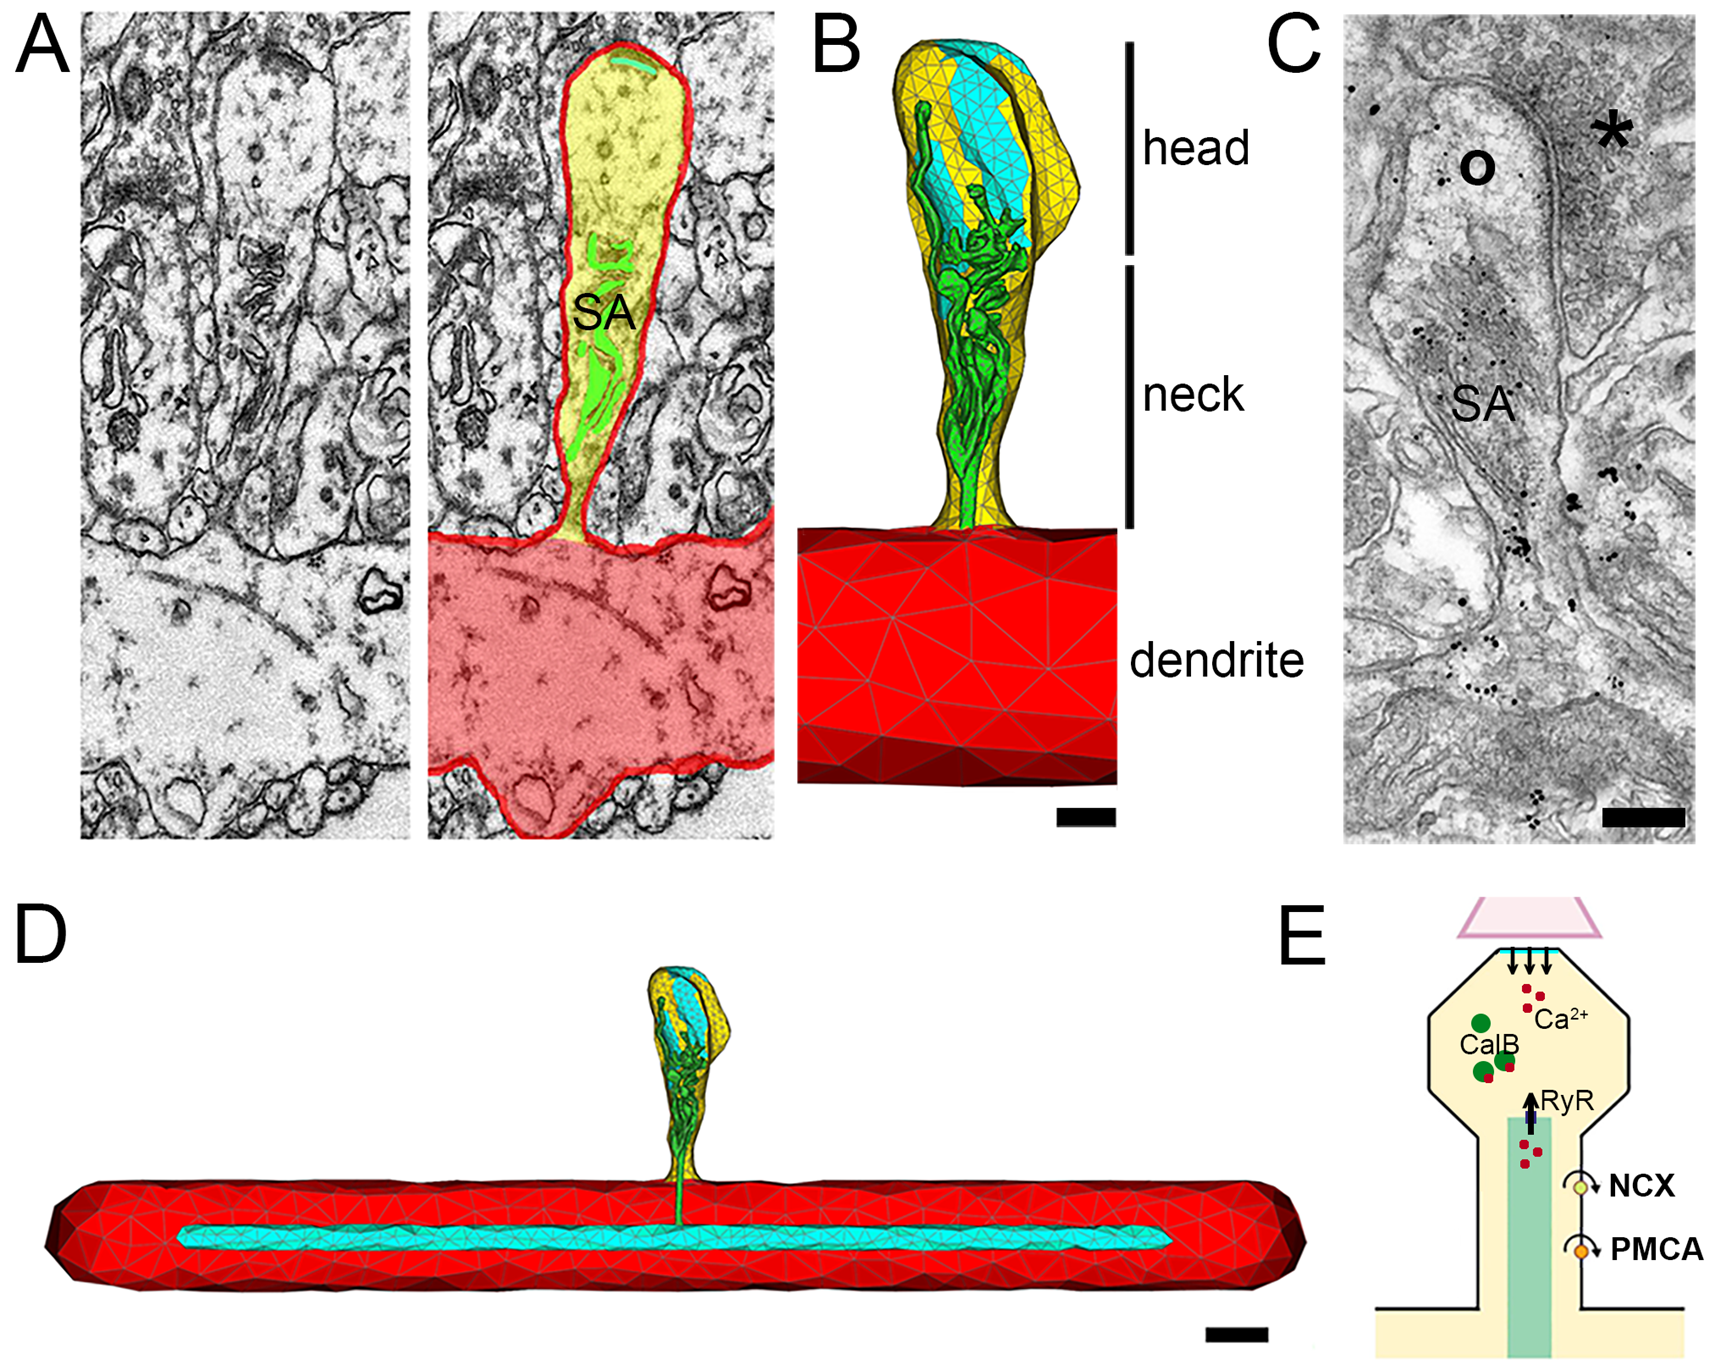
\includegraphics[width=0.7\textwidth]{images/figure1.png}
\caption{{\small\textbf{Dendritic spine reconstruction and Ca2+ modeling.} (A) Spine morphologies are based on serial reconstructions of transmission electron micrographs obtained from human cortical tissue. (B) An example of a reconstructed dendritic spine (dendrite, red; spine compartment, yellow) carrying a spine apparatus organelle (SA, green). Upon release of Ca2+ at the reconstructed postsynaptic density (cyan), changes in [Ca2+] are determined in the head, neck and dendritic region, respectively. Scale bar, 200 nm. (C) Immunogold staining for the actin-binding protein synaptopodin, which is a marker and essential component of the SA. Asterisk indicates presynaptic, circle the postsynaptic  compartment. Scale bar, 200 nm. (D) In all reconstructed human spines the SA was attached to a single standardized dendritic ER tubule in a dendritic compartment with identical dimensions. Scale bar, 500 nm. (E) The model accounts for Ca2+ exchange mechanisms on the plasma membrane (Na+/Ca2+ exchangers (NCX), plasma membrane Ca2+ ATPases (PMCA)) and on the ER (green; ryanodine-receptors (RyR)). Calcium buffering capacity (Calbindin, CalB) is kept constant. Further details are provided in the main text and in Tables xxx. See also supplemental movie.}}
\end{figure}

\section*{Results}
\subsection*{Spine Ca2+ modeling in reconstructed human dendritic spines containing a spine apparatus organelle}
To capture the effect of the SA on Ca2+ dynamics in dendritic spines, the three-dimensional architecture of dendritic spines, including intracellular membrane structures, must be carefully considered. Extending on the results obtained from synthetically generated dendritic spines (Breit et al. 2018) the detailed morphologies of 9 dendritic spines, their SA and postsynaptic densities (PSD) were reconstructed from cortical surgical access material using serial transmission electron microscopy (TEM). From serial TEM image stacks realistic three-dimensional geometric models were generated (Figure 1A, B).

Immunogold staining for the actin-binding protein synaptopodin, which is an essential component for the formation of the SA in the rodent brain (Deller et al., 2003; Vlachos et al., 2013), confirmed that synaptopodin is a marker for the human SA (Figure 1C; c.f., Lenz et al., 2020). The reconstructed SAs were then attached to a single standardized dendritic ER tubule in a dendritic compartment of identical dimensions for all spines (Figure 1D). The resulting surface triangulation of the plasma membrane, the SA, the PSD, and dendritic ER were then used to construct a volumetric tetrahedral mesh for numerical simulations. 

Existing single-channel models of Ca2+ exchangers in the plasma membrane, i.e., plasma membrane Ca2+ ATPase (PMCA) and Na+/Ca2+ exchangers (NCX), as well as Ryanodine receptors (RyR) on the SA membrane (see schematic in Figure 1E) were adapted and integrated into a diffusion-reaction model for cytosolic and endoplasmic Ca2+ dynamics (c.f., Breit et al., 2018). Numerical simulations were carried out on computational domains defined by the reconstructed human dendritic spine morphologies, using established numerical methods (details provided in Methods).

We recently showed that ~70\% of all dendritic spines on layer II/III pyramidal neurons contain a synaptopodin cluster, i.e., SA (Lenz et al., 2021). By carefully examining EM cross sections we also obtained evidence that large human dendritic spines contain SA organelles (Lenz et al., 2021), which is consistent with earlier work on synaptopodin clusters and spine head sizes of hippocampal neurons prepared from the rodent brain (Okubo-Suzuki et al., 2008; Vlachos et al., 2009; Yap et al., 2020). However, it has remained unclear whether, among SA containing human dendritic spines, larger spines also contain larger SAs and PSDs. Although, it has been shown that spines with SA had higher head volumes and neck diameters than spines without SA (Ofer et al., 2021). 

\begin{figure}[h!]
\centering
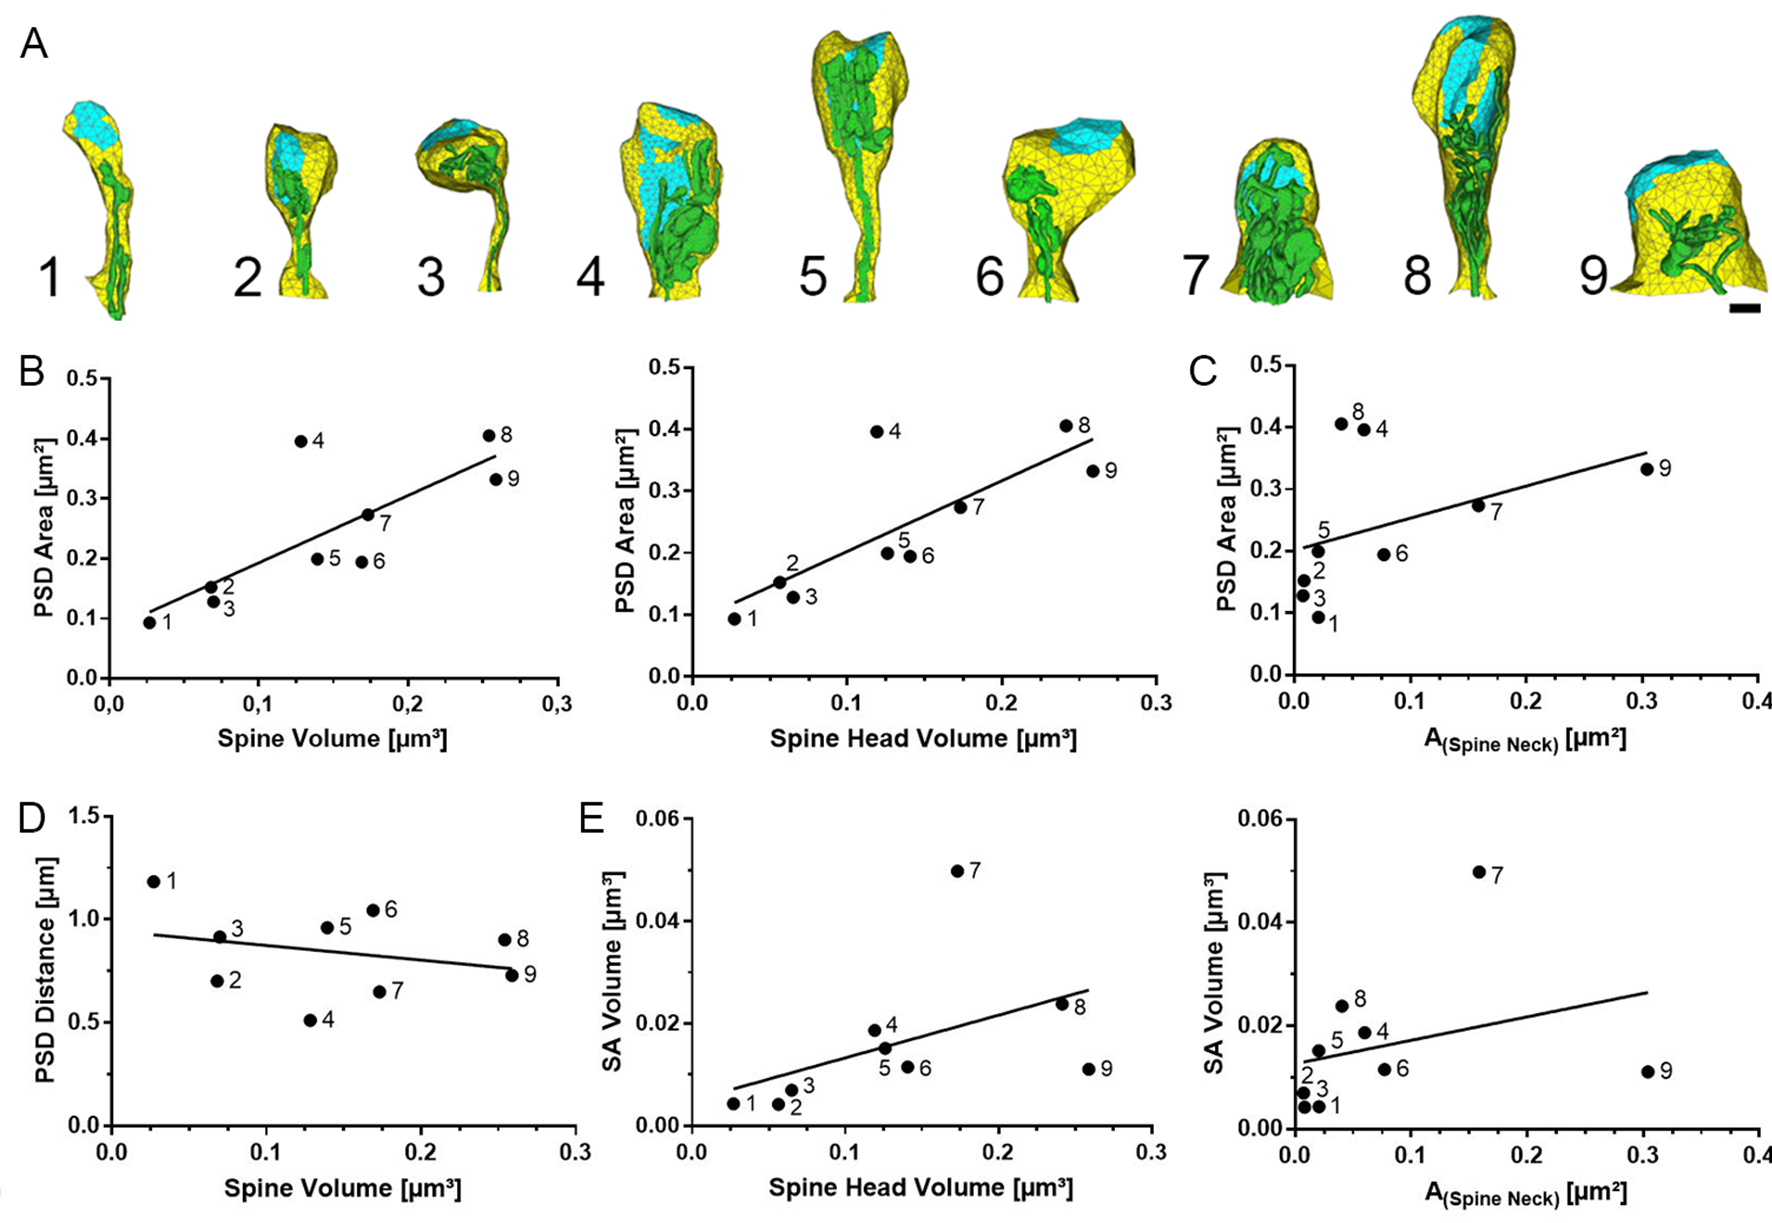
\includegraphics[width=0.9\textwidth]{images/figure2.png}
\caption{{\small\textbf{ Morphological parameter of reconstructed spines.} (A) Three-dimensional models based on reconstructed human dendritic spines. Spine apparatus organelle, green. Postsynaptic density, cyan. Scale bar, 200 nm (B) Dendritic spines with large volumes have large postsynaptic densities. (C) Positive correlation between spine neck diameter and postsynaptic density sizes (D) Postsynaptic densities in large spines are not further away from spine base. (E) Large spines contain large spine apparatus organelles, which are found in spines with wider spine necks. n = 9 reconstructed dendritic spines from 4 independent samples.}}
\end{figure}

To test whether there are correlations between the reconstructed spine components, we carefully examined critical morphological parameters of the reconstructed SA-containing dendritic spines (Figure 2). Consistent with previous studies in animal models (Harris et al., 1989; Arellano et al., 2007) a positive correlation between PSD sizes and spine volumes was observed in the spines reconstructed from human cortical tissue (Figure 2A, B). This relation was readily detected when spines were sorted by spine head volumes. Moreover, a positive correlation between PSD sizes and cross-sectional area of spine necks was observed (Figure 2C). This finding raises the intriguing possibility that large spines with a wide neck may allow for a more effective Ca2+ spine-to-dendrite communication.
Considering the major scope of this study, i.e., modeling of spine-to-dendrite Ca2+ communication, we determined distances between PSDs and the dendritic compartment. Figure 2D shows no significant correlation between spine volumes and PSD-to-dendrite distances, which were defined as the Euclidian distance between the point of the PSD closest to the base of the spine. These results indicate that SA-containing spines of the human cortex may differ in their volume and spine neck diameters, while PSD-to-dendrite distances are comparable, at least for the 9 reconstructed spines used in this study.

Finally, we examined morphological properties of the SAs contained in the reconstructed spines (Figure 2E). A positive correlation was observed between spine volumes and SA volumes, which was also observed when spine neck cross-sections were considered. These results provide ultrastructural morphological insight into the three-dimensional organization of SA-containing dendritic spines in the human cortex (c.f., Lenz et al., 2021). They support the previously proposed spine-within-a-spine ER morphology, that is a critical role of spine volume and sER volume ratio in Ca2+ signaling (c.f., Bell et al., 2019). 

\begin{figure}[h!]
\centering
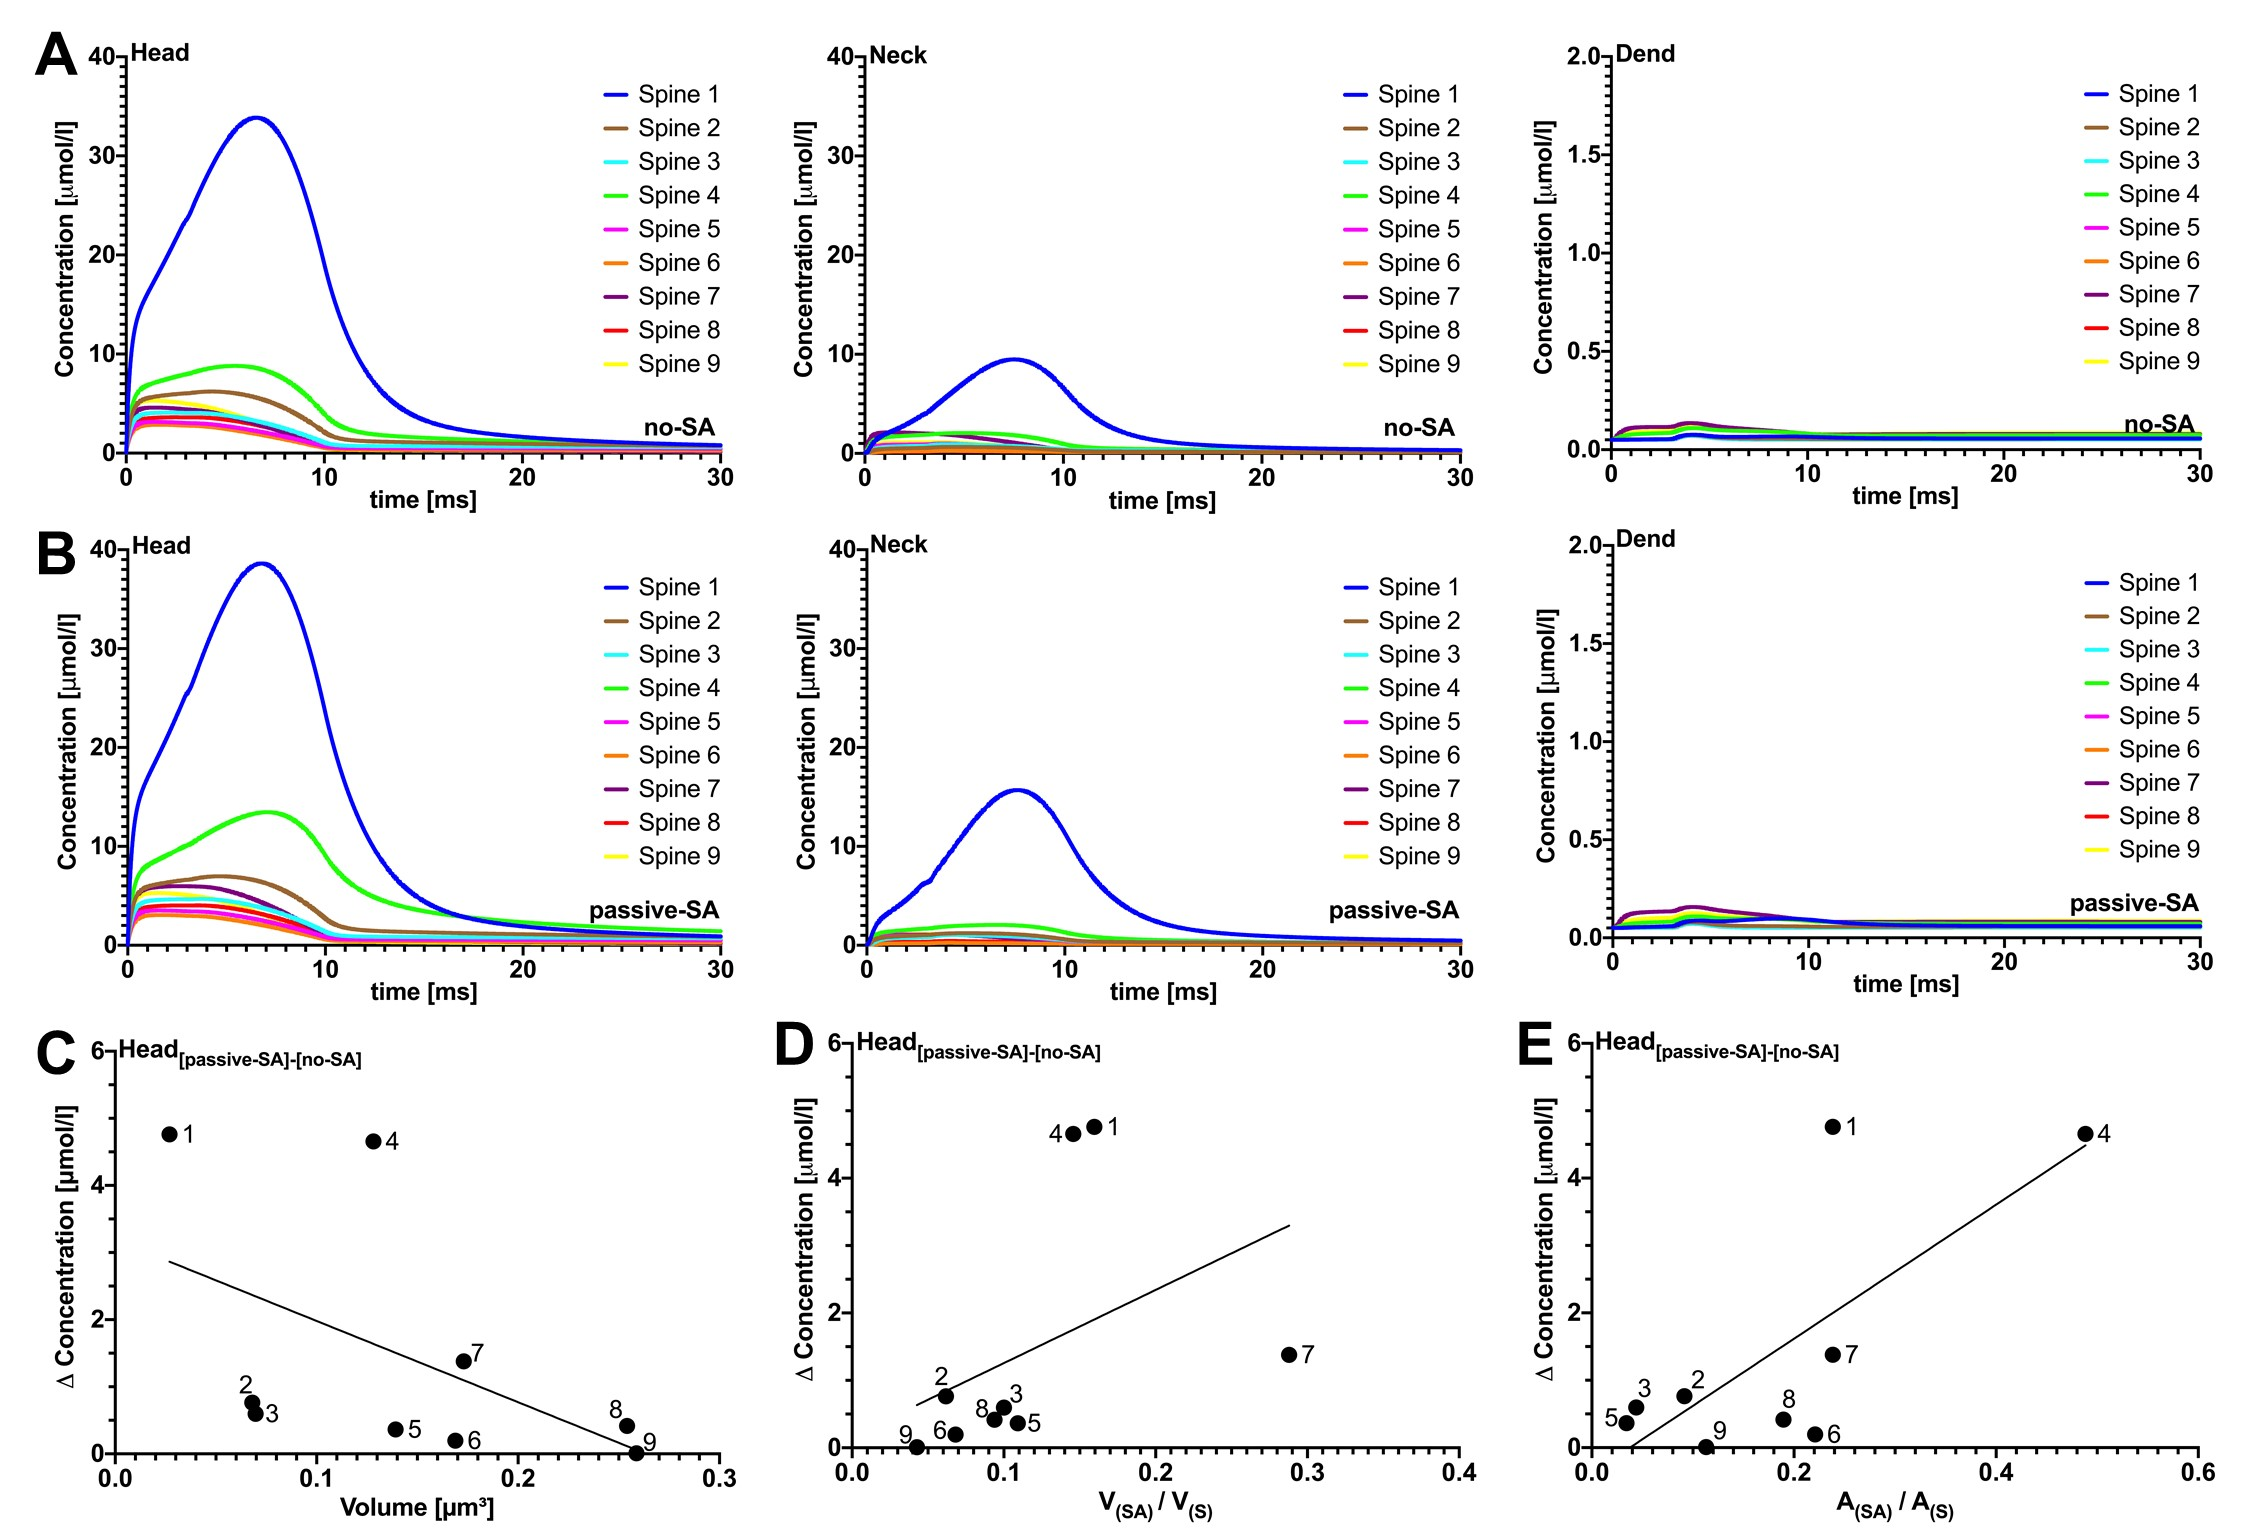
\includegraphics[width=0.9\textwidth]{images/figure3.jpg}
\caption{{\small\textbf{ Effects of passive spine SA on spine-to-dendrite Ca2+ signaling, with fixed Ca2+ influx.}  Plots A1-A3 (without  SA) and B1-B3 (with SA) show Ca2+ profiles for 10 ms initial Ca2+ release into the spine head.  Consistent with experimental data, spine-to-dendrite Ca2+ signaling does not occur for all 9 simulated spines, and this also holds true for simulations where Ca2+ influx is adapted to the postsynaptic area, see additional plots. Plots C1-C3 (fixed Ca2+ influx) demonstrates correlations between maximum [Ca2+ ] in the head region versus spine volume, ratio of SA area/ Spine area, and SA volume/ Spine volume. Presence of a passive SA, i.e., no Ryanodine or IP3 receptors, has no major effect on Ca2+ dynamics in the spine head and neck.}}
\end{figure}

\subsection*{Passive SA organelles have no major impact on spine-to-dendrite Ca2+ signaling} To assess the role of the SA in spine-to-dendrite Ca2+ communication, we first investigated Ca2+ signal propagation in spines for which the reconstructed SA was excluded. In all simulations the same number of Ca2+ ions were released into the spine head at the respective PSD (Sabatini et al., 2002; Keller et al., 2008; Higley et al., 2012) and changes in [Ca2+] were measured in three regions of interest: the spine head, spine neck and the dendrite (Breit et al., 2018).

As shown in Figure 3A, only a small fraction of released Ca2+ ions reaches the dendritic compartment. To quantify the dendritic response to Ca2+ release at the PSD, the [Ca2+] amplitude was measured in the spine head, neck and dendrite. The values and ratios between head and dendrite amplitude for all spines are listed in Table 2. In all cases less than 3\% of the initial [Ca2+] amplitude in the head was detectable in the dendrite. When the SA was added as a passive compartment, i.e., when it was present as a geometric obstacle, but without any Ca2+ exchange mechanisms that would allow Ca2+ exchange across the SA membrane, similar and near-zero dendritic [Ca2+] profiles are observed in the respective spines (Figure 3B). Minor differences in the profiles (compared to the no-SA case) can be observed in the head and neck, however these all lie in the single digit µmol/l range.

The differences in peak [Ca2+] amplitude between passive-SA and no-SA are presented in Figure 3C–E. These differences decrease with increasing spine volume (Figure 3C) and are positively correlated to the SA/Spine volume ratio (Figure 3D). Two clear outliers in this trend are spine 1 and 4. To test whether the SA has the ability to block calcium passage at the intersection between head and neck and thus produce larger differences in the [Ca2+] amplitude, the data was plotted against the SA/Spine surface area ratio at this intersection (Figure 3E). The outlier spine 4 could clearly be explained by this metric. Thus, accumulation of SA in the intersectional region between head and neck (‘corking’ effect) could obstruct [Ca2+] diffusion. Numerical simulations were also carried out for PSD adjusted Ca2+ influx (see Supplemental Figure 7), i.e. Ca2+  influx was scaled by PSD surface area, using spine 8 as the reference spine. It should be noted that PSD adjusted Ca2+ influx may compensate for the Ca2+ accumulation in the head region. In Supplemental Figure 7(C1) for instance the change in [Ca2+] remains relatively uniform when correlated against spine volume, with the exception of spine 4 for which we observe the above described “corking effect”. Taken together, from these results (fixed Ca2+ and PSD adjusted) we conclude that spine-to-dendrite Ca2+ signaling in the dendrite is negligible for the no-SA and the passive-SA setting. These observations strengthen the case for active Ca2+ exchange across the spine ER membrane to enable spine-to-dendrite Ca2+ communication in SA containing dendritic spines.

\begin{figure}[h!]
\centering
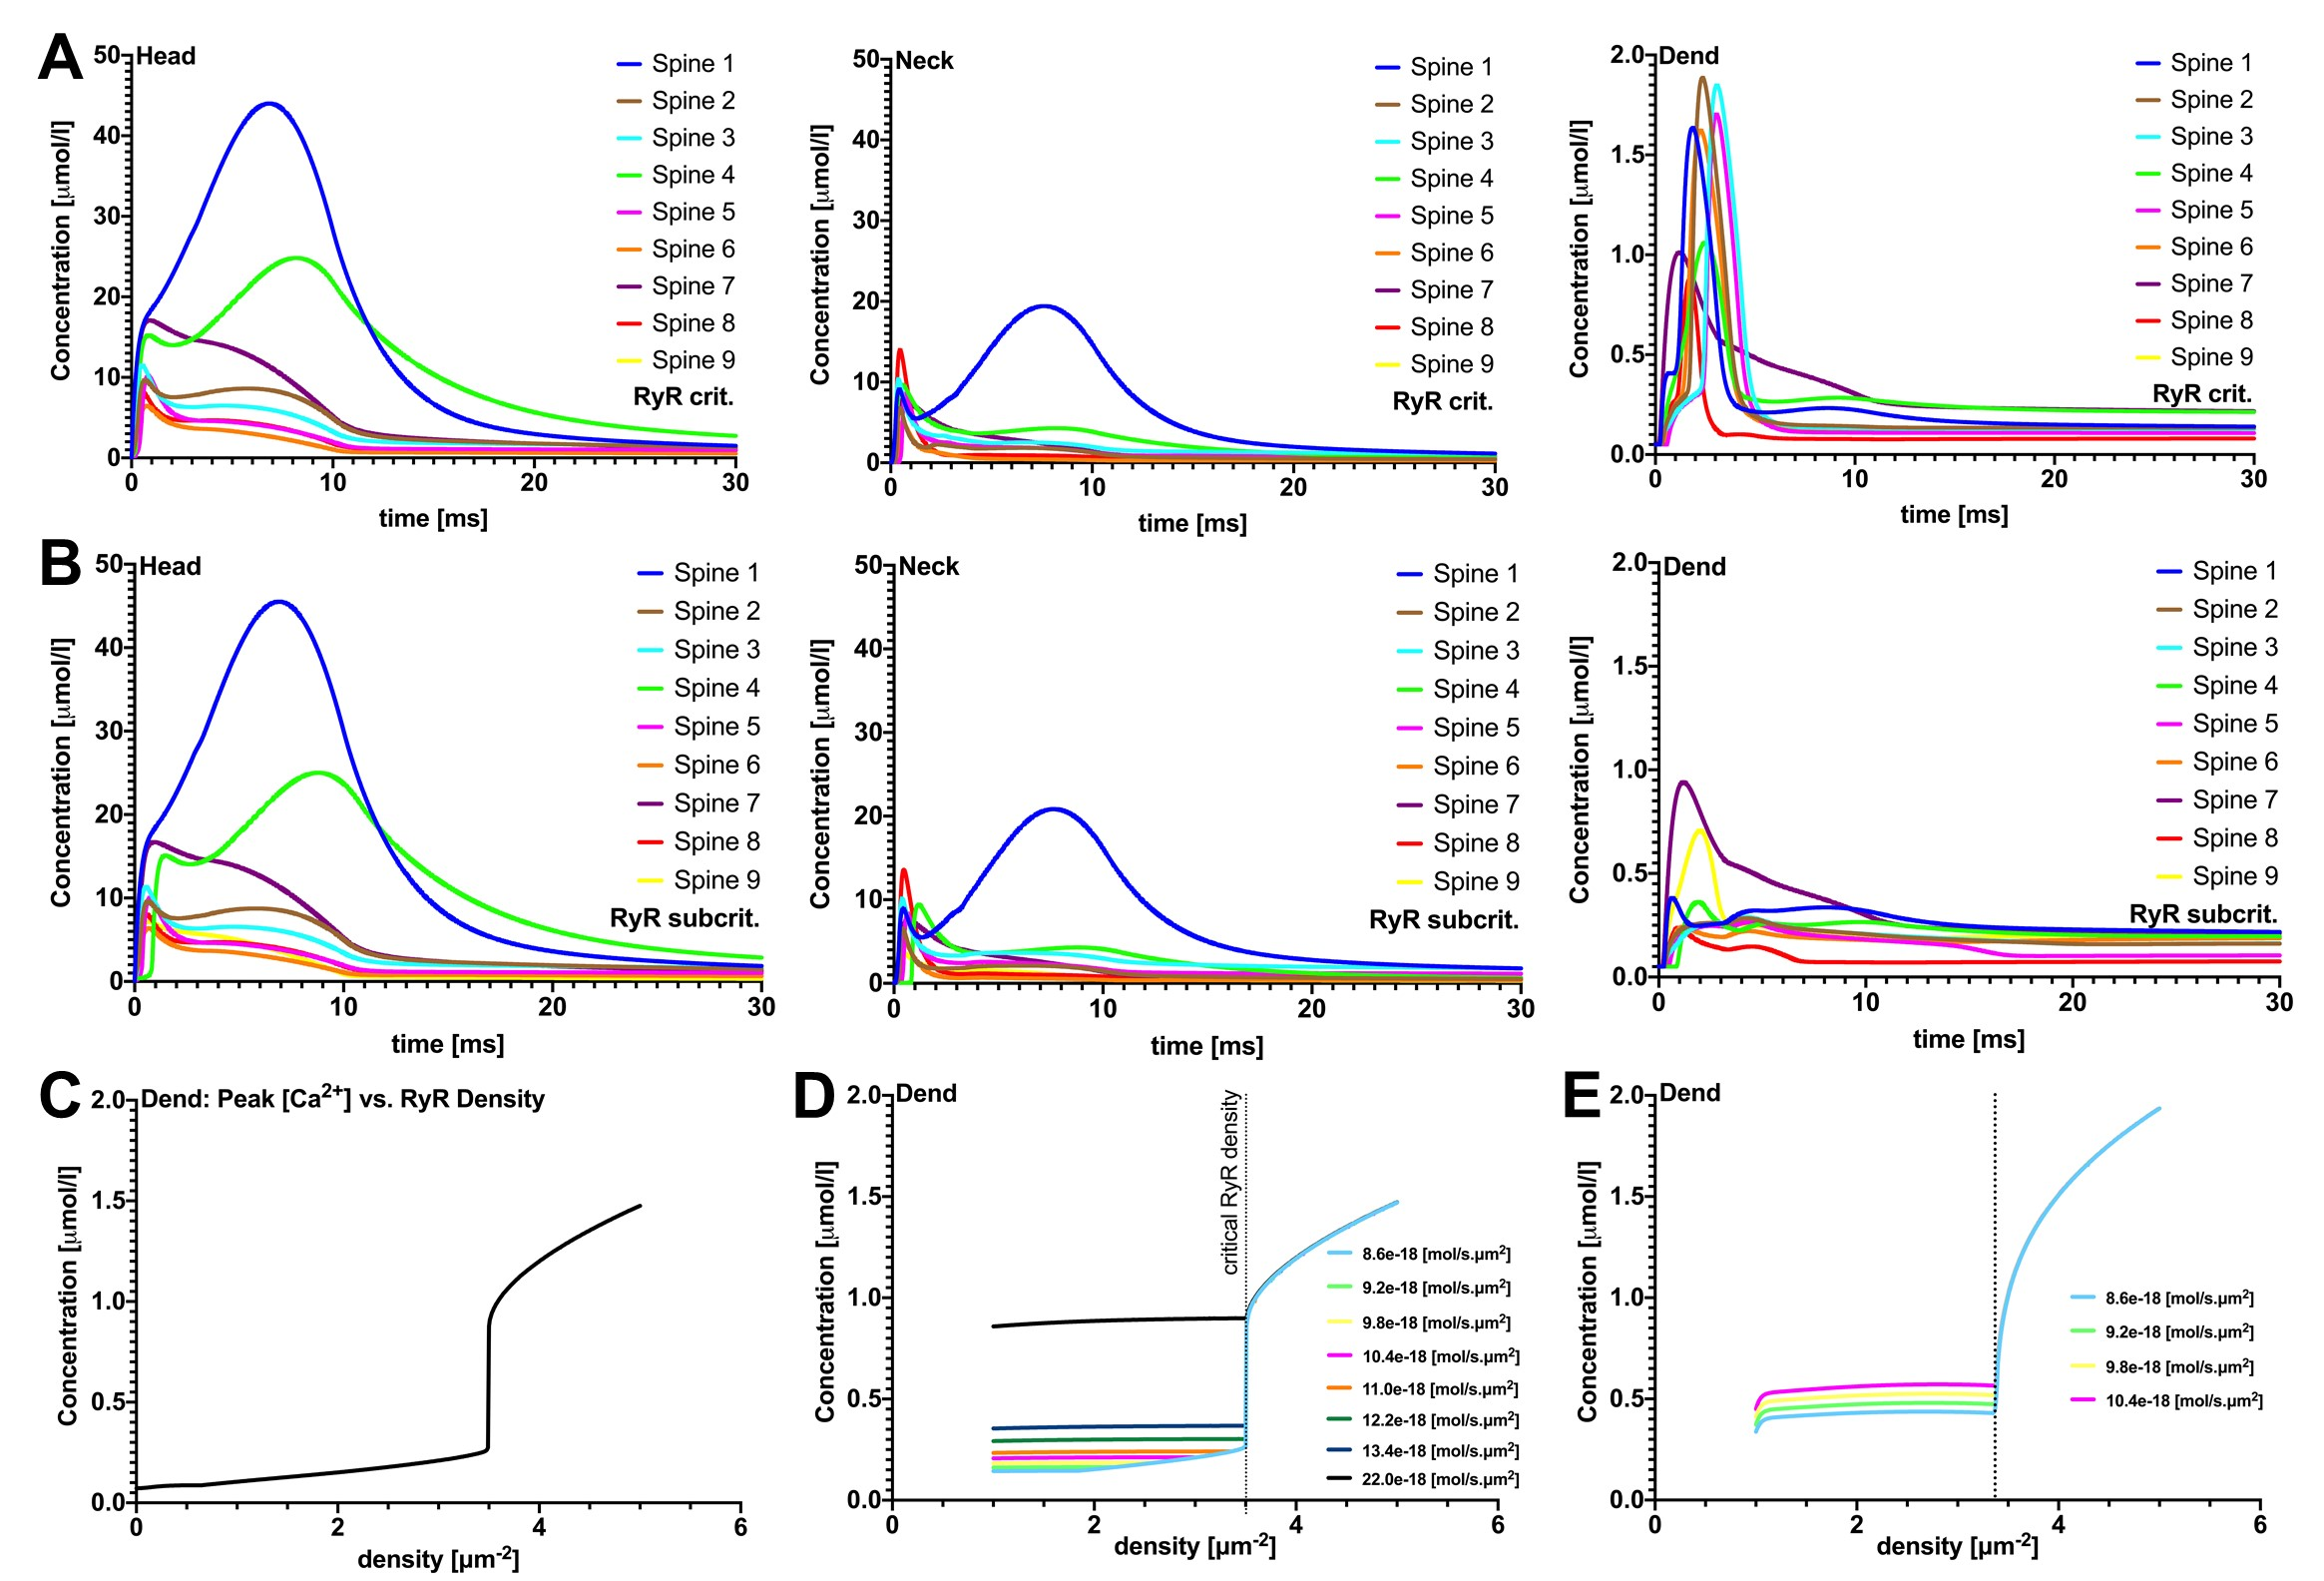
\includegraphics[width=0.9\textwidth]{images/figure4.jpg}
\caption{{\small\textbf{Effects of active SA with RyR calcium exchange mechanisms only.} These plots were generated with active SA with only ryanodine receptors. For the plots in row A, these are the calcium concentration traces in the head and dendrite regions at the critical RyR density. For the plots in row B, these are the calcium concentration traces at sub-critical (5\% below critical) RyR density, observe that Ca2+ coupling is significantly decreased. For Figures 4C-E, we demonstrate for spine 8, there is a critical RyR density  such that Ca2+ coupling occurs in the dendritic region. The RyR density parameter is incremented at 0.01 um-2 increments, observe the maximum [Ca2+] in the dendritic region has a significant jump at ~ 3.50 um-2. For plot D we performed the same RyR density increment experiments but with different Ca2+ influx at the synapse. For all spine simulations (rows A and B) we used a fixed Ca2+ influx at the synapse, i.e. for every spine the same calcium influx value was used.}}
\end{figure}

\subsection*{Ryanodine receptor density of SA controls spine-to-dendrite Ca2+ signaling} Previous work revealed that RyR dependent Ca2+-induced Ca2+ release from synaptopodin associated Ca2+ stores modulates spine Ca2+ dynamics and synaptic plasticity (Vlachos et al., 2009; 2013; Korkotian et al., 2014). To assess the role of active SAs, by including RyRs on the membrane of the SA and dendritic ER, the RyR density critical for spine-to-dendrite Ca2+ coupling was determined for each spine (Figure 4). To quantify coupling, we defined a peak [Ca2+] > 1 µmol/l in the dendritic measuring zone for 1 ms, with conversion this leads to 1e-18 mol/s.µm3 and multiply by the width of the dendrite (~1 µm) to obtain an approximate flux through the neck-dendritic interface of 1e-18 mol/s.µm2, i.e., >11\% of initial Ca2+ influx at the PSD using 8.6e-18 mol/s.µm2,  as successful spine-to-dendrite coupling. We increased the RyR density in 0.01/µm2 increments in the range of 0–5 RyRs per µm2 and found critical RyR values for all reconstructed morphologies, ranging between 1.37-3.5/µm2 (Table 1). Figure 4A shows that all spines elicit dendritic Ca2+ coupling when the critical RyR density is surpassed. However, the peak [Ca2+] drops below 1 µmol/l when the RyR density is subcritical (Figure 4B). Thus, RyR density plays a critical role in spine-to-dendrite coupling.

We next tested whether changes in calcium entry at the PSD affect the critical RyR density by successively increasing the Ca2+ flux density at the PSD entry site. However, coupling occurs at the same RyR density, independent of the initial Ca2+ influx within the range 8.6e-18--22.0e-18 mol/s.µm2 tested here (Figure 4C-4D). This invariance can be attributed to intracellular Ca2+ buffering, as modifications in the buffering capacity produced a shift in the critical RyR density. This was observed when we ran our simulations with half the buffering capacity, Figure 4E, causing a decrease in the critical RyR density. It is worth pointing out that the transition between coupling and decoupling spine-to-dendrite Ca2+ signals is highly nonlinear (see jumps in Figure 4C-E). With control over critical RyR density appear to have the ability to control all-or-nothing Ca2+ dynamics in the parent dendrite.

Comparing the peak [Ca2+] concentrations of passive and active SA in head and dendrite (see Table 2) shows that the relative differences between passive and active ER dynamics are the result of Ca2+-induced Ca2+ release through RyRs, which releases additional Ca2+ into the cytosol. While the critical RyR density was not dependent on Ca2+ influx at the PSD, we further studied whether the intracellular organization may play a role. 

\begin{figure}[h!]
\centering
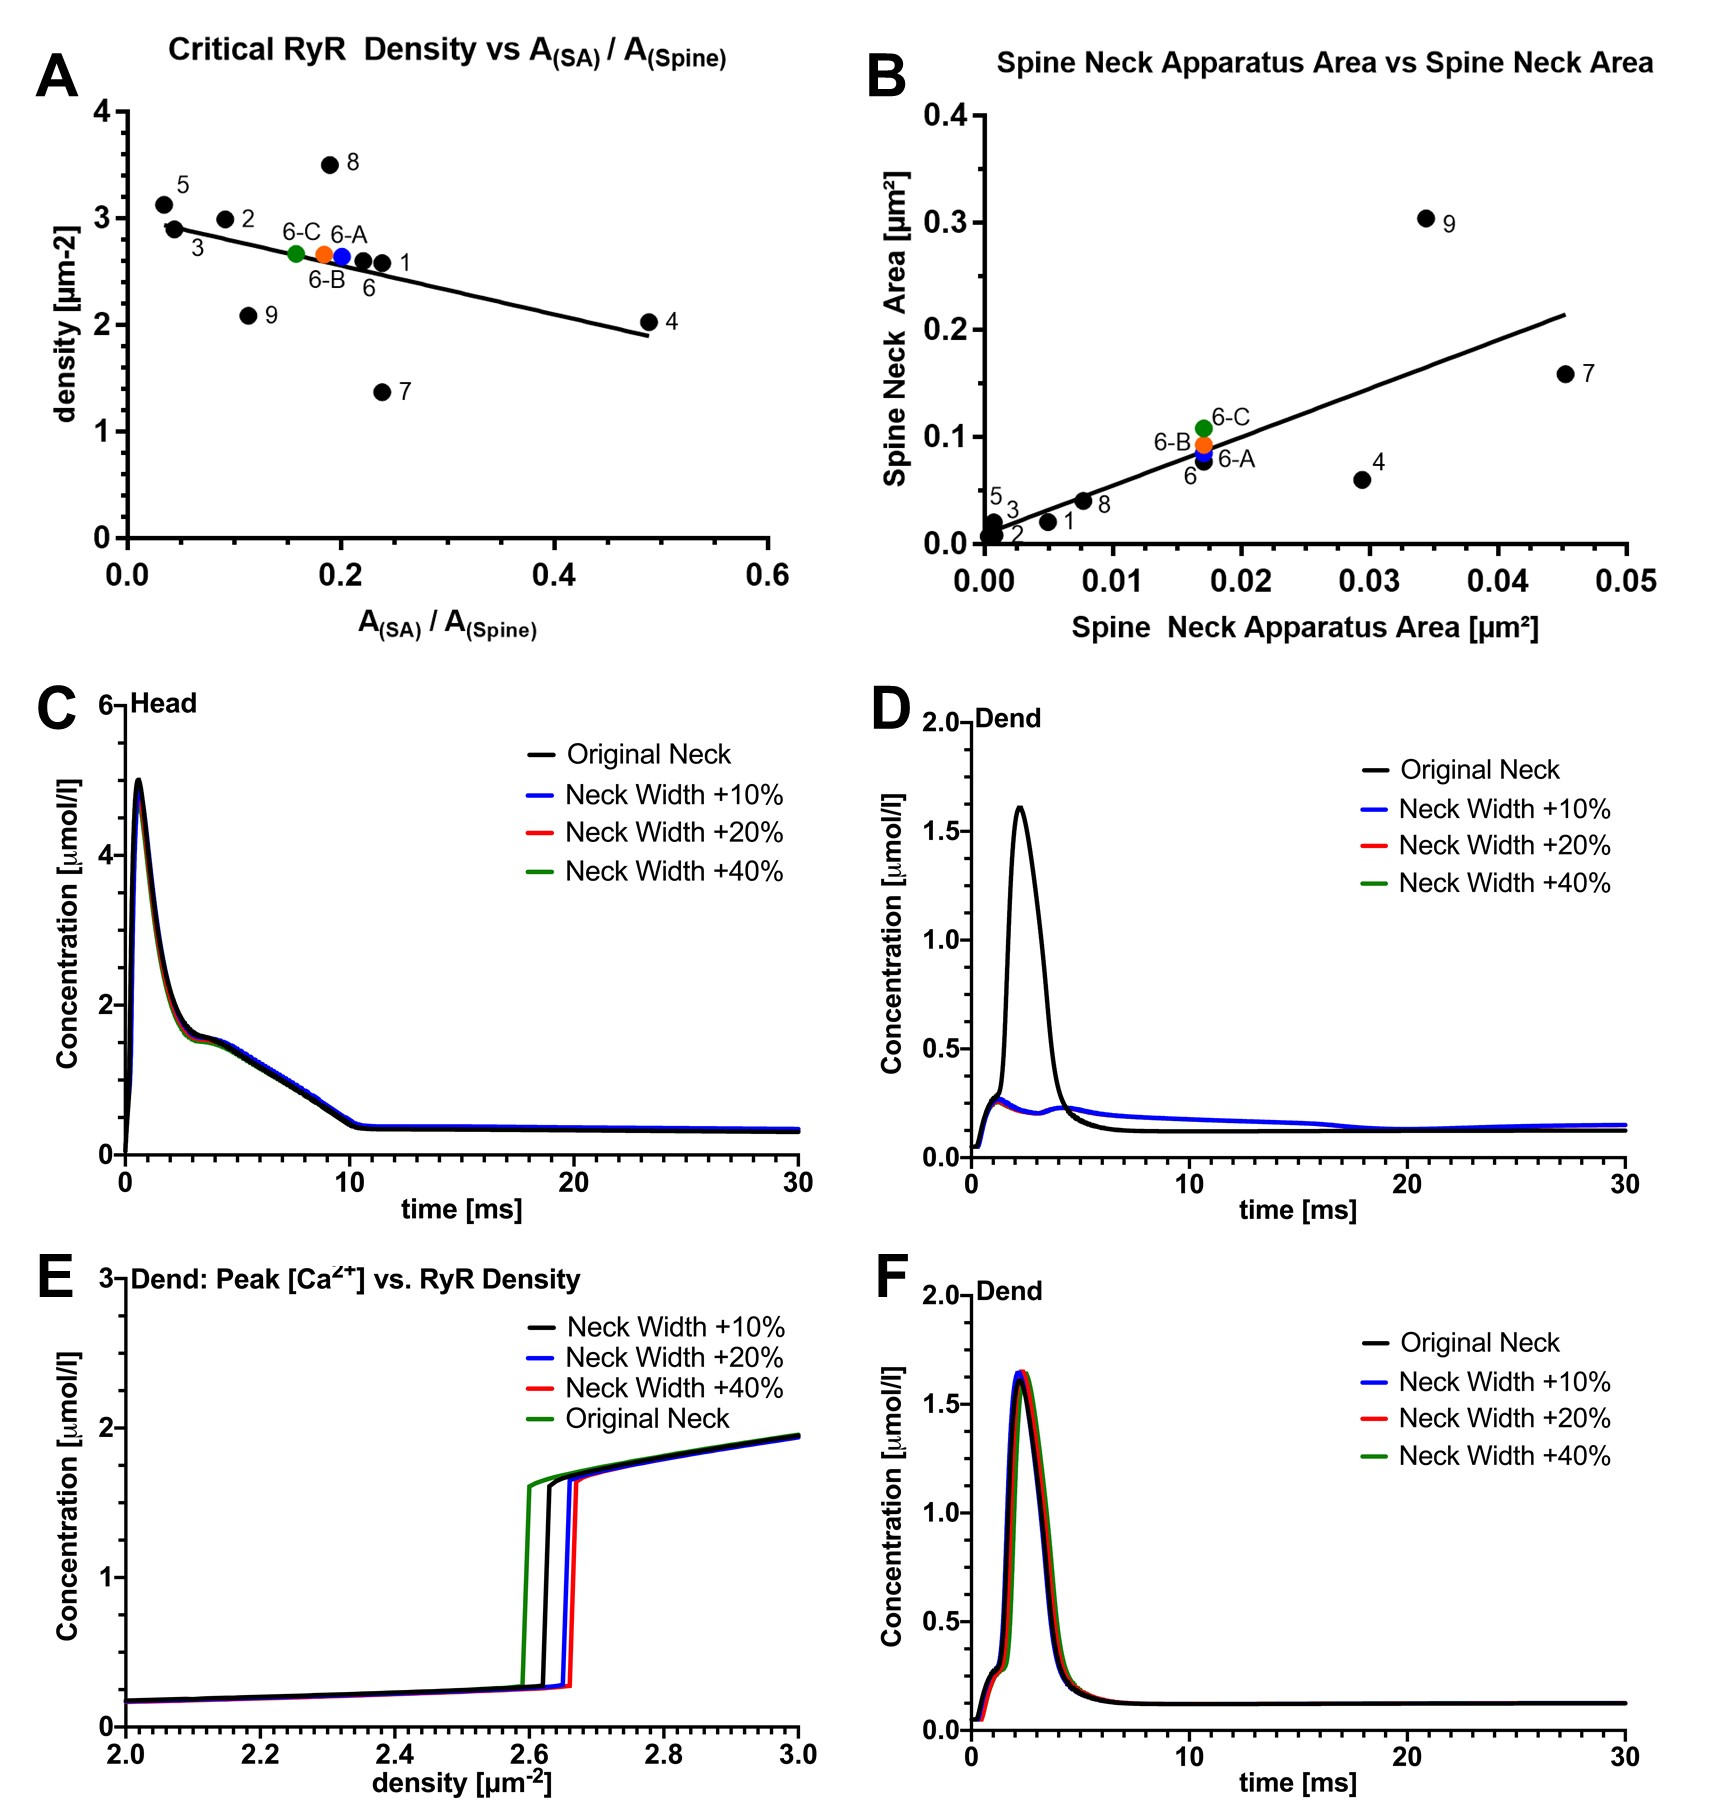
\includegraphics[width=0.8\textwidth]{images/figure5.jpg}
\caption{{\small In figure 5.A we plot the critical RyR density agains the ratio of Spine Apparatus Neck area to Spine Neck area. In Table 1 we show the values that correspond to figure 5.A. In figures 5.C -5.D we demonstrate that widening the neck diameter of a spine affects the coupling of Ca2+ to the dendritic region. In particular figure 5.E indicates that neck widening causes the critical RyR density to increase.}}
\end{figure}

\subsection*{Spine morphology and neck plasticity affect spine-to-dendrite Ca2+ signaling}Critical for endoplasmic Ca2+ release through RyRs is sufficient [Ca2+] at the endoplasmic membrane (REF). Thus, an intracellular organization of the SA that would support sufficient accumulation of Ca2+ at the spine neck (the most confined part of the spine morphology) should decrease the critical RyR density. To test this hypothesis, the critical RyR density was plotted against the ratio of SA in the spine-neck to spine-neck cross-sectional area (Figure 5A). We found that the area ratio correlated negatively with the RyR density, demonstrating that a smaller RyR density is sufficient to induce spine-to-dendrite coupling when the SA occupies larger portions of the spine neck.

		To highlight this correlation we reference spine 4 (Figure 2A shows that the SA lies tightly at the interface of spine head and neck), which produces a sharp and pronounced release of Ca2+ in the dendritic shaft (Figure 4C). In comparison, spine 5 (Figure 2A shows that the SA forms only a thin tubule from head to dendrite) produces a more gradual Ca2+ change, which can be attributed to the absence of substantial Ca2+ accumulation at the SA membrane.
		
		Interestingly, we observed a positive correlation between spine and SA cross-sectional area of the spine neck (Figure 5B), suggesting that the SA follows dendritic spine growth and reorganizes in such a way to support spine-to-dendrite communication. In fact, previous work has demonstrated that changes in spine neck diameters accompany the induction of excitatory synaptic plasticity, reflected by an increase in spine head size. Specifically, spine necks are shortened and widened after long-term potentiation of excitatory neurotransmission (Tønnesen et al., 2014). 
		
		We therefore systematically tested whether changes in spine neck diameter can affect spine-to-dendrite Ca2+ communication. To address the role of spine neck plasticity in spine-to-dendrite Ca2+ communication we ran simulations by using the reconstruction of spine 6 and manually widening the spine neck by 10, 20, and 40\%, while keeping the RyR density and the SA morphology constant (Figure 5, modified spines 6-A, 6-B, 6-C, respectively). While the Ca2+ dynamics in the spine head remain unchanged (Figure 5C), we observed that increasing the spine neck width caused a decrease in peak Ca2+ near the SA membrane, therefore producing insufficient Ca2+ release from the SA store to maintain spine-to-dendrite coupling (Figure 5D). 
		
		We then tested whether an increase in RyR density could balance morphology plasticity in order to maintain coupling even under spine growth and reorganization. For each of the modified spines 6-A, 6-B, and 6-C we incrementally increased the RyR density and observed that a critical RyR density can be determined for all spines. Naturally, this critical value increases with increasing neck width, see Figure 5E (critical RyR densities for spines 6-A, 6-B, 6-C can be found in Table 1). 
		
		Not only could coupling be restored but, as Figure 5F shows, the dendritic calcium profiles for all adjusted spines are nearly identical. This indicates that [Ca2+] is sensitive to changes in spine neck and SA morphology i.e. Ca2+ diffusion is affected by spine neck and SA geometry (Svoboda, Tank, Denk; 1996). In conclusion, we observed an all-or-nothing communication switch between spine head and dendrite that is controlled by an interplay between RyR density and plasticity of spine morphology. 


\section*{Discussion}

In this study we explored spine Ca2+ dynamics in human cortical spines using simulations consisting of Ca2+ diffusion and reaction with mobile calcium buffer (calbindin) in the cytosol, Ca2+ diffusion inside the SA and sER of the dendrite, as well as Ca2+ exchange across the plasma (PMCA, NCX) and endoplasmic (RyR) membranes (Figure 1). We show that a critical RyR density, dependent on the overall spine and SA architecture, allows active CICR release to maintain spine-to-dendrite Ca2+ communication. By increasing the neck diameter or decreasing the spine apparatus cross-sectional area in the neck region or individual spines this communication pathway is disrupted. Increasing the RyR density can reverse this effect (Figure 8). These findings suggest a critical role of SA- and spine neck plasticity in controlling all-or-nothing Ca2+ communication between the spine head and dendrite.

	The ability to visualize individual dendritic spines in living brain tissue over extended periods was introduced three decades ago (Guthrie, Segal \& Kater 1991; Müller \& Connor, 1991). Consequently, the amount of information about morphology and physiology of dendritic spines and the molecular mechanisms acting on spines has tremendously increased (please cite Svoboda, Sabbatini, Holtmaat, Oertner, Sala \& Segal). Yet, major issues regarding structure-function interrelations and the role of dendritic spines in network function and memory mechanisms remain unsettled (Segal 2017). This is particularly true for structure-function interrelations in the adult human cortex. It is currently not possible to simultaneously visualize (1) dendritic spine morphology, (2) presence and precise position of spine ER, i.e., the spine apparatus, and (3) in releasing reproducible amounts of Ca2+ while (4) carrying out Ca2+ imaging at high temporal and spatial resolution in living human cortical tissue. Also, it is currently impossible to systematically assess the relevance of individual spine and ER parameters, as they are not easy to manipulate in biologically complex systems. To start better understanding spine Ca2+ dynamics in human cortical neurons we employed computer simulations based on serial TEM reconstructions.

	Our morphological analysis of the 9 reconstructed spines used in this study confirms and extends findings from a recent study on synaptic plasticity of layer II/III pyramidal neurons in human cortical access material (Lenz et al., 2021). In this earlier study we showed that approximately 70\% of dendritic spines contain synaptopodin clusters; (2) synaptopodin clusters and spine apparatus organelles are found in large dendritic spines; and (4) a plasticity-inducing stimulus promotes remodeling of synaptopodin clusters, spine apparatus organelles, and dendritic spines in cortical slices prepared from the adult human brain. These changes correlated well with changes in spontenous excitatory postsynaptic currents recorded from individual layer II/III pyramidal neurons. Consistent with these earlier findings, a positive correlation between SA volume, spine volumes and PSD sizes is established. Likewise, we confirmed that synaptopodin is a marker for the human spine apparatus organelle (Figure 1X). While we have to concede that this analysis is based on 9 reconstructed spines only, disclosing such interrelation with comparably small numbers indicates that these morphological measures are tightly regulated in human cortex. It likely that icnreased use of new electron microscopy techniques such as focused ion beam, block face serial electron microscopy and array tomography, together with computer based automatic 3D reconstructions will allow us to…


\section*{Methods}

\subsection*{Ethics Statement}Human brain tissue was obtained from a local biobank operated in the Department for Neurosurgery at the Faculty of Medicine, University of Freiburg Germany (AZ 472/15\_160880). All procedures were carried out after positive evaluation by the local ethics committee (AZ 593/19). 

\subsection*{Electron Microscopy}
Tissue was fixed in 4\% paraformaldehyde ($w/v$) and 2\% glutaraldehyde ($w/v$; phosphate buffered saline) overnight. After fixation tissue was cut into 100 $\mu$m thin slices, thoroughly washed in phosphate buffer (0.1M) and incubated with 1\% osmium tetroxide for 60 minutes. After washing in graded ethanol (up to 50\% $v/v$) for 10 minutes each, slices were incubated with uranylacetat (1\% ($w/v$) in 70\% ($v/v$) ethanol) overnight. Slices were then dehydrated in graded ethanol (80\%. 90\%, 96\% for 10 minutes each, and 2x 100\% for 10 minutes). After two washing steps in propylenoxide for each 5 minutes each slice was incubated with durcupan/propylenoxid (1$:$1 for 1 hour) following durcupan only overnight at room temperature. Ultrathin sections of 20 - 40 nm were prepared at a Leica UC6 Ultracut. Sections were mounted into copper grids (Plano) and contrasted using Pb-citrate for 3 minutes. Transmission electron microscopy was performed at a Zeiss Leo 906 equipped at 6000x magnification. In total cortical access tissue from 7 individuals who underwent clinically indicated neurosurgical procedures, e.g., for tumors or epilepsy, were processed and 1 to 6 acquisitions were obtained from each patient. Each acquisition included at least one labeled dendritic segment and synaptic contact. Up to 40 images of the same dendritic spines on consecutive sections were acquired and saved as TIF-files. 

\subsection*{3D-reconstrunction of dendritic spines and generation of spine models} Image series were adjusted in brightness and contrast using the Fiji software package (Schindelin et al., 2012). Stack alignment and segmentation were performed with the integrated TrakEM2 plugin (Cardona et al., 2012). For this purpose, an automatic alignment (rigid registration) was utilized followed by manual correction. Independent traces were drawn manually for each spine attached to a dendritic segment, spine apparatus organelles and postsynaptic densities. Dendritic spines possessing spine apparatus organelles that were complete within the series were reconstructed. A total of 9 series met these criteria and were used in analysis. The image segmentation binary files were transformed into a preliminary surface mesh using the Java 3D library (Schmid et al., 2010). However, meshes generated in this manner contained various mesh artifacts as jagged boundaries, non-manifold features and surface intersection. Using the meshing software ProMesh (Reiter et al., 2013) according to a post-processing scheme, conditioned surface meshes were produced which are compatible with physical simulations. Mesh defects such as disconnects in the spine apparatus organelle due to thickness in ultrathin section or error in segmentation were counterbalanced by manual identification and matching of cellular structures. All reconstructed spines including their spine apparatus organelles were cut from their parent dendritic shaft through the base of the spine neck. Subsequently, they were attached to an dendritic segment containing the endoplasmatic reticulum. Elaborating this method, we inserted realistic shapes of spine apparatus into reconstructed human spine models and generated hybrids of actual anatomical morphologies with simplified geometries. Using ProMesh, we directly measured volumes from the three-dimensional reconstructions. While spine neck length was measured from the center of the spine head base towards the insertion of the spine to the dendrite, neck diameter was calculated as an average diameter from three measurements obtained proximal, intermediate and distal to the edge of the dendrite. Linear regressions were performed by best-fit approaches and were statistically tested to be different from zero with the statistical software GraphPad Prism (GraphPad Software).
\subsection*{Calcium Simulations} All necessary components were implemented in the simulation toolbox NeuroBox (Breit et al., 2016). NeuroBox is a simulation toolbox that combines models of electrical and biochemical signaling on one- to three-dimensional computational domains. NeuroBox allows the definition of model equations, typically formulated as ordinary and partial differential equations, of the cellular computational domain and specification of the mathematical discretization methods and solvers (Reiter et al., 2013; Vogel et al., 2013). 
\subsection*{Model Equations}
\subsection*{Membrane Transport Equations}

\subsection*{Numerical Methods}
For numerical simulations, the four equations are discretized in space using a finite volumes method. Current densities, both synaptic and across the ER and plasma membranes, can be incorporated into the reaction-diffusion process very naturally and easily this way. We show how this is achieved using the cytosolic Ca2+ Eq. (3) as an example: It is reformulated (using the divergence theorem) to an integral version 

(integral equation)

where B is a control volume that will be specified shortly, and [PUT EQUATION HERE] is the outward normal on the boundary of B. For control volumes located at the ER membrane, some portion of its boundary will coincide with the ER membrane. Since there is no diffusive flux density [put equation here] across the ER membrane, we can simply substitute it by the ER flux density jERM as given in (7) in the boundary integral for this portion of the boundary. The same applies to the plasma membrane and the synapse area. Te diffusive flux is set to zero on the rest of the cytosolic domain
boundary. If we denote the cytosolic boundary by [A SYMBOL], its ER/plasma membrane and synaptic parts by [PUT SYMBOLS HERE], respectively, this yields the following equation:
(integral equation)
Control volumes are constructed as a Voronoi-like dual tesselation of the original tetrahedral mesh by connecting the mid-points of edges, faces and volumes through planar facets. Equation (27) must hold for all control volumes, giving rise to one equation per control volume.
Time discretization is realized using a backwards Euler scheme, i.e., for each point in time t, the term [PUT EQUATION HERE] in (27) is replaced by the discretized term [putEQUATION HERE] and all quantities on the right-hand side are evaluated at time t. Here, [PUT SYMBOL HERE] is the time step size of the time discretization. By limiting the function space to the space of continuous functions that are linear on all volumes of the original mesh, the integrintegrals in Eq. (27) can be evaluated efficiently. Moreover, the solution can be represented by one degree of freedom per volume, so there is one equation for each degree of freedom. The system of equations arising from this procedure is nonlinear (due to the nonlinear reaction term and, more importantly, the highly nonlinear transport terms across the membranes) and is therefore linearized by a Newton iteration.
For the results we present here, the emerging linearized problems were solved using a Bi-CGSTAB linear solver using Gauss-Seidel preconditioning. Computations were facilitated by a domain decomposition parallelization approach and carried out using the UG 4 framework.

\nocite{*}
\bibliography{sample.bib}

\section*{Acknowledgements}

We thank Sigrun Nestel for excellent technical assistance in transmission electron microscopy. This work was supported by a Collaborative Research in Computational Neuroscience Grant (CRCNS; NIH and BMBF; xxxxxxxxx to GQ, 01GQ1804A to AV).
\clearpage
\section*{Tables}
\begin{table}[h!]
    \centering
    \begin{tabular}{|c|c|}
    \hline
        \textbf{Spine No.} & \textbf{RyR Critical Density $[\mu m^{-2}]$} \\ \hline
        1 & 2.58 \\ 
        2 &2.99 \\ 
        3 &2.9 \\ 
        4&2.03 \\ 
        5&3.13 \\ 
        6&2.6 \\ 
        6A&2.64 \\ 
        6B&2.66 \\ 
        6C&2.67 \\ 
        7&1.37 \\ 
        8&3.5 \\ 
        9&2.09 \\ \hline
    \end{tabular}
    \caption{}
\end{table}


\begin{table}[h!]
\begin{tabular}{|c|c|c|c|c|c|c|}
\hline
\textbf{\begin{tabular}[c]{@{}c@{}}Spine\\  No.\end{tabular}} & \textbf{\begin{tabular}[c]{@{}c@{}}Head - passive\\  peak {[}Ca2+{]} µmol/l\end{tabular}} & \textbf{\begin{tabular}[c]{@{}c@{}}Head - active\\  peak {[}Ca2+{]} µmol/l\end{tabular}} & \textbf{\begin{tabular}[c]{@{}c@{}}\% Head\\  increase\end{tabular}} & \textbf{\begin{tabular}[c]{@{}c@{}}Dendrite - passive\\  peak {[}Ca2+{]} µmol/l\end{tabular}} & \textbf{\begin{tabular}[c]{@{}c@{}}Dendrite - active \\ peak {[}Ca2+{]} µmol/l\end{tabular}} & \textbf{\begin{tabular}[c]{@{}c@{}}\% Dendrite \\ increase\end{tabular}} \\ \hline
1                                                             & 33.85                                                                                     & 44                                                                                       & 30\%                                                                 & 0.08                                                                                          & 1.64                                                                                         & 1950\%                                                                   \\
2                                                             & 6.22                                                                                      & 9.66                                                                                     & 55\%                                                                 & 0.07                                                                                          & 1.89                                                                                         & 2600\%                                                                   \\
3                                                             & 4.09                                                                                      & 11.47                                                                                    & 180\%                                                                & 0.07                                                                                          & 1.85                                                                                         & 2543\%                                                                   \\
4                                                             & 8.8                                                                                       & 24.82                                                                                    & 180\%                                                                & 0.11                                                                                          & 1.06                                                                                         & 864\%                                                                    \\
5                                                             & 3.16                                                                                      & 10.22                                                                                    & 223\%                                                                & 0.07                                                                                          & 1.7                                                                                          & 2329\%                                                                   \\
6                                                             & 2.86                                                                                      & 6.47                                                                                     & 126\%                                                                & 0.07                                                                                          & 1.62                                                                                         & 2214\%                                                                   \\
7                                                             & 4.6                                                                                       & 17.09                                                                                    & 270\%                                                                & 0.14                                                                                          & 1.01                                                                                         & 621\%                                                                    \\
8                                                             & 3.62                                                                                      & 8.11                                                                                     & 124\%                                                                & 0.07                                                                                          & 0.88                                                                                         & 115\%                                                                    \\
9                                                             & 5.29                                                                                      & 7.2                                                                                      & 36\%                                                                 & 0.12                                                                                          & 1.05                                                                                         & 775\%                                                                   \\ \hline
\end{tabular}
\caption{}
\end{table}

\clearpage
\section*{Supplemental Figures}
\begin{figure}[ht!]
\centering
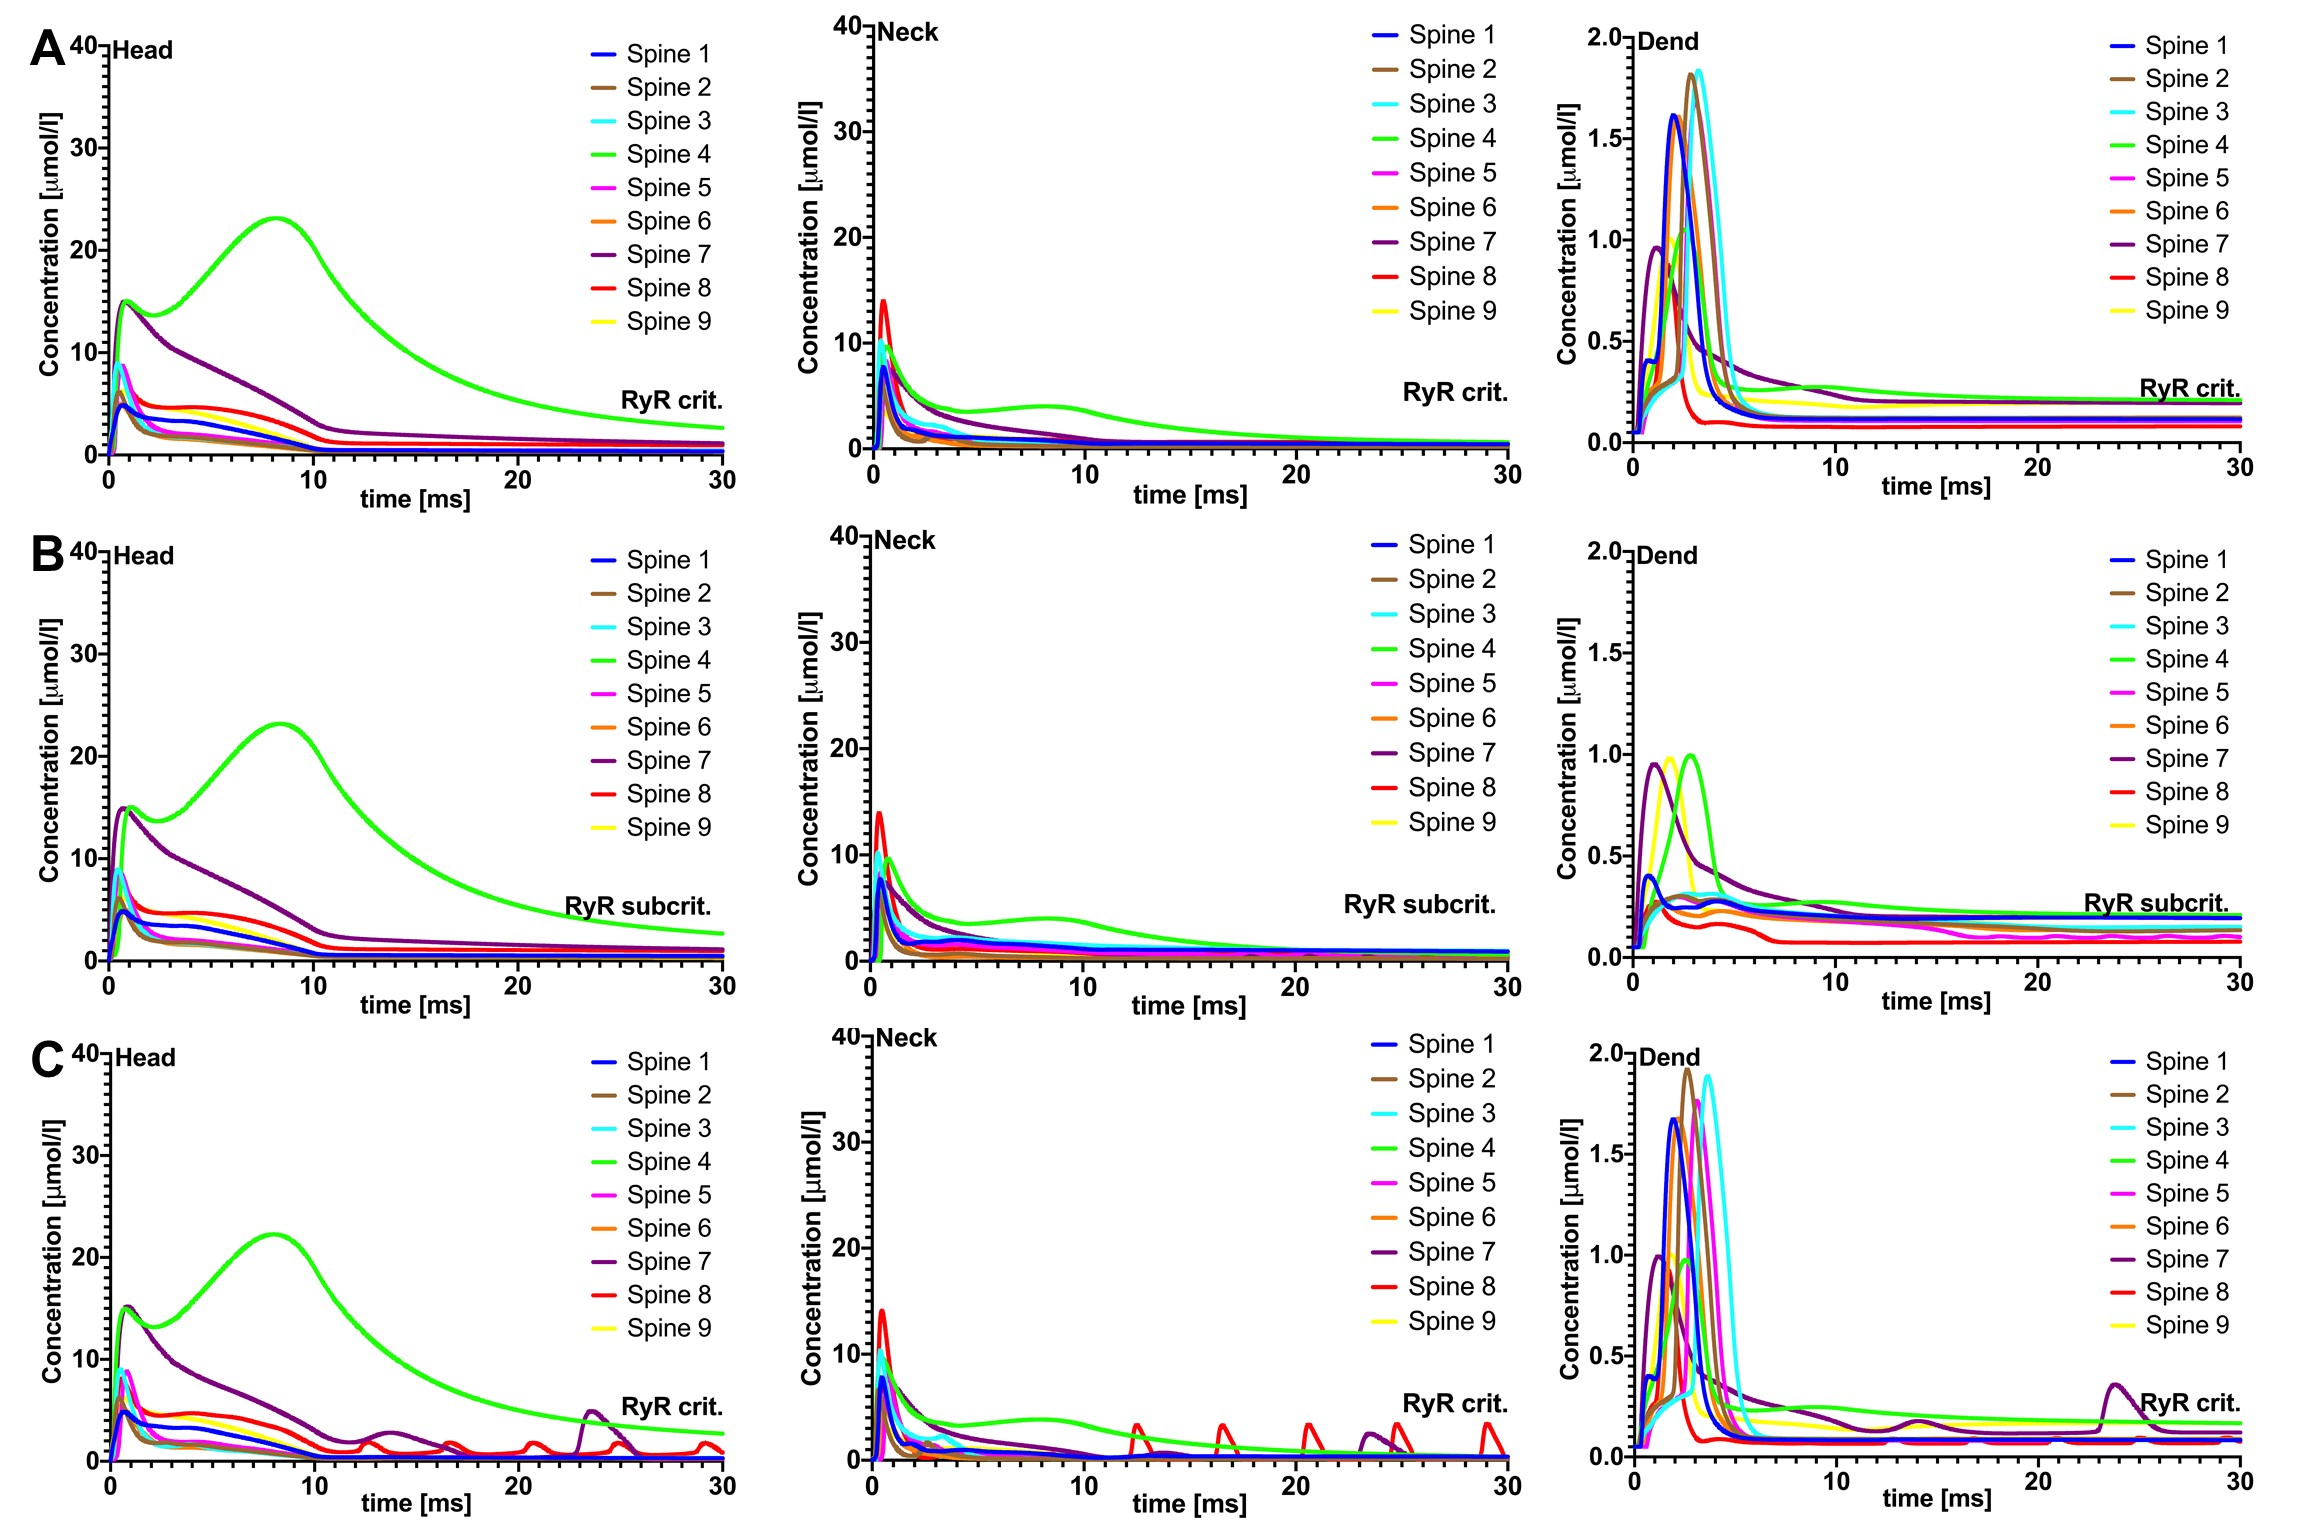
\includegraphics[width=0.9\textwidth]{images/figure6.jpg}
\caption{{\small All plots in figure 4 were generated with PSD adjusted calcium influx. In row A, these are the calcium concentration profiles in the head and dendrite region with SERCA pumps off and at critical RyR density. In row B, these calcium concentration profiles correspond to sub-critical RyR density. In row C, these are the calcium concentration profiles at critical RyR density with SERCA pumps on. In row C, when SERCA pumps are activated we observe oscillations in the some of the calcium concentration profiles}}
\end{figure}

\begin{figure}[ht!]
\centering
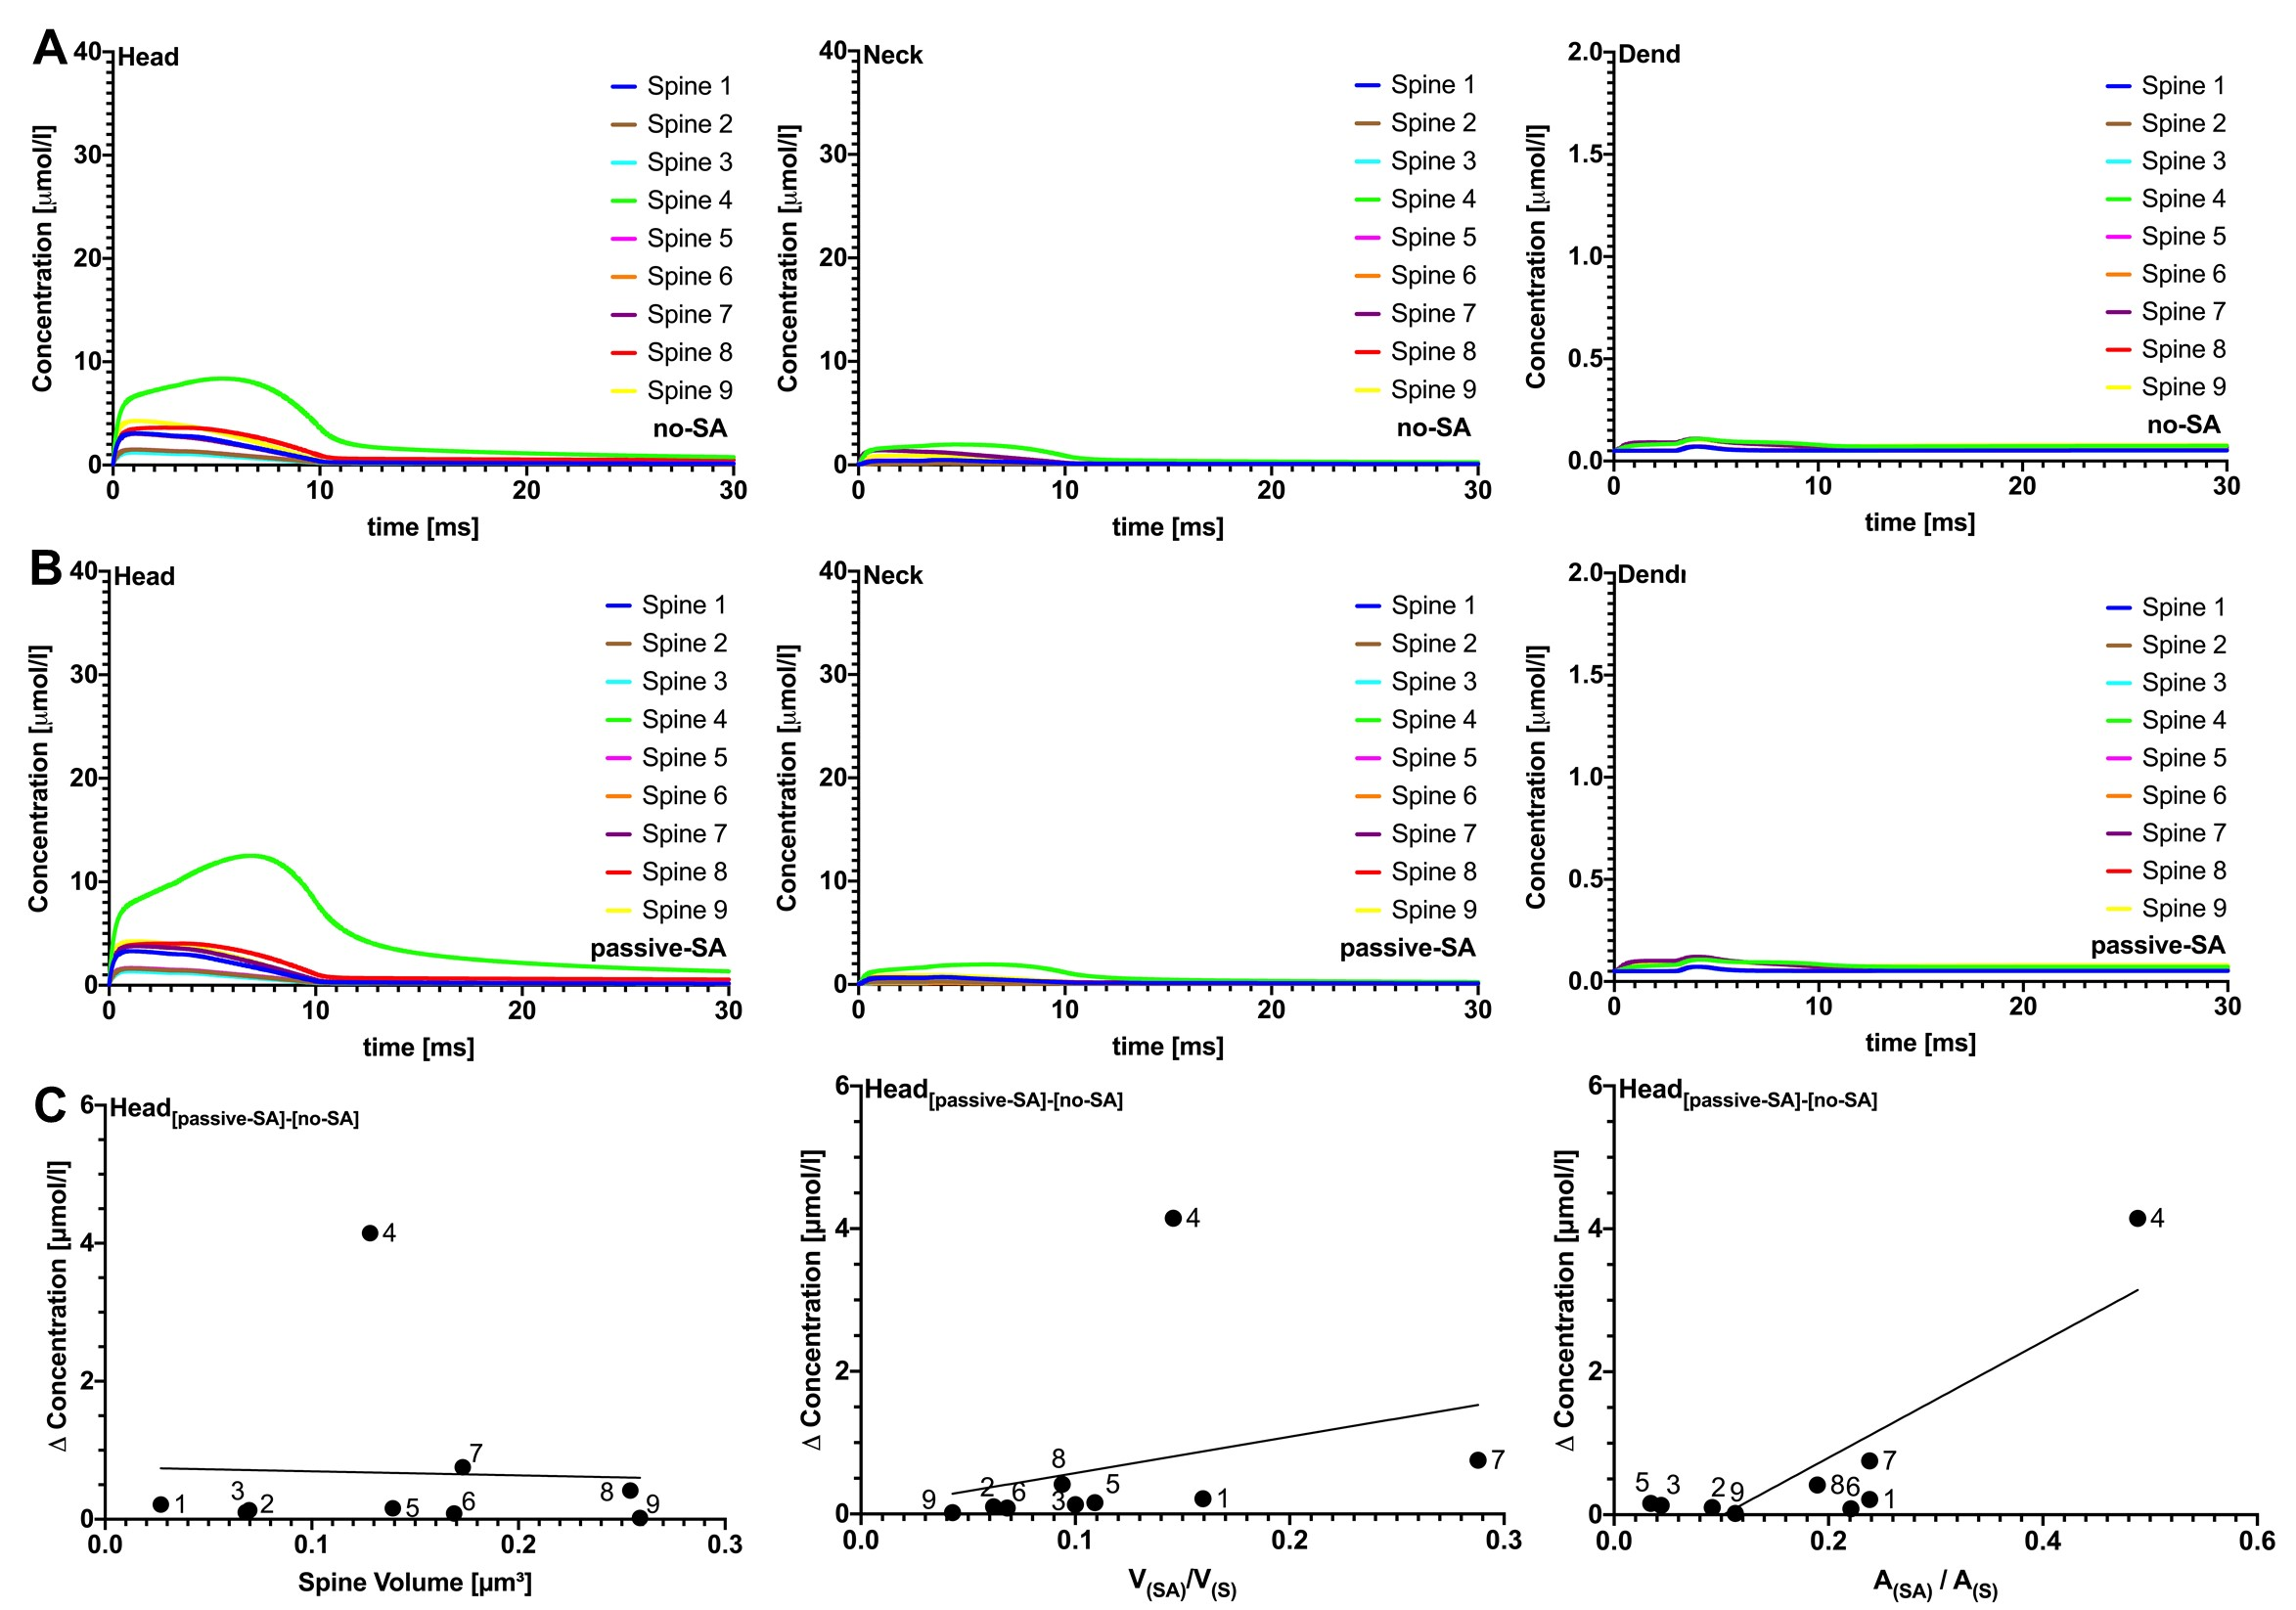
\includegraphics[width=0.9\textwidth]{images/figure7.jpg}
\caption{{\small Figure 7: Effects of passive spine SA on spine-to-dendrite Ca2+ signaling, with PSD adjusted Ca2+ influx.  Plots A1-A3 (without  SA) and B1-B3 (with SA) show Ca2+ profiles for 10 ms initial Ca2+ release into the spine head.  Consistent with experimental data, spine-to-dendrite Ca2+ signaling does not occur for all 9 simulated spines. Presence of a passive SA, i.e., no Ryanodine or IP3 receptors, has no major effect on Ca2+ dynamics in the spine head and neck.}}
\end{figure}

\end{document}